\section{バイメタル小片の熱構造解析}
この例では、バイメタルの小片が、各層の異なる熱膨張のために曲がります。
モデルは、2本の梁(120$\times$20$\times$4mm)を互いに重ねて配置したもので構成されています。
\begin{enumerate}
\item
  {[}mm, ton, s, °C{]}単位の新規ファイルを作成し、ステップ形式のジオメトリをPrePoMaxにインポートします。
  次に、両方のパーツをメッシュ分割します。
  ここでは、両方のパーツの最大要素サイズを1mmとし、その他の設定は変更しませんでした(図\ref{fig:12-01})。
	\begin{figure}[H]
	\centering
	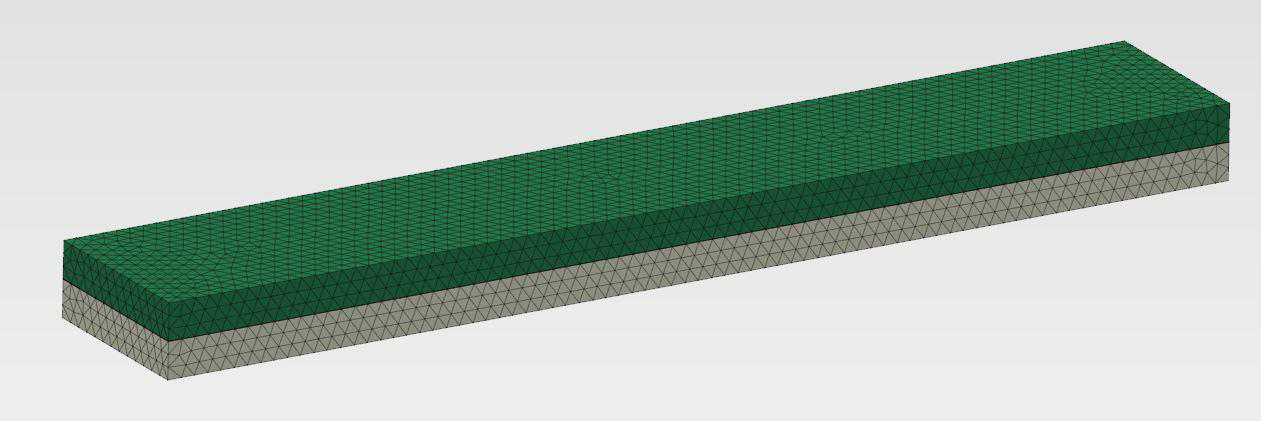
\includegraphics[width=145mm]{fig/12-01.png}
	\caption{バイメタル小片 - メッシュ}
	\label{fig:12-01}
	\end{figure}
	\vspace{-\baselineskip}
\item
  Copperという名前の新しい材料を定義し、弾性(ヤング率130000MPa、ポアソン比0.34)、熱伝導率(385mW/(mm・°C))、熱膨張率(17e-6(1/°C)、零温度20°C)を追加します。
  別の材料を定義し、名前をSteelとし、弾性(ヤング率21000MPa、ポアソン比0.3)、熱伝導率(45mW/(mm・°C))、熱膨張率(12.3e-6(1/°C)、零温度20°C)を追加します。
  材料にCopperを使用し、Top\_layerという名前のソリッドセクションを新規に作成し、そのセクションが割り当てられるように上部の梁を選択します。
  別のセクションを作成し、名前をBottom\_layerとし、材料にSteelを選び、下の梁を選択します。
\item
  上部の梁を非表示にし、下部の梁の上面にTie1という名前のサーフェスを作成します。
  パーツの可視性を反転させ(View → Invert Visible Parts)、上部梁の下面にTie2という名前のサーフェスを作成します。
  再び両方のパーツを表示します。
  タイ拘束を定義し、以前に作成したサーフェスをマスターとスレーブ領域として使用します。
\item
  温度-変位連成解析ステップをデフォルト設定(定常状態)で定義します。
\item
  両方の梁の背面に固定境界条件を割り当てます。
  固定された面以外のすべての外面に、80℃の温度境界条件を追加します(図\ref{fig:12-02})。
	\begin{figure}[H]
	\centering
	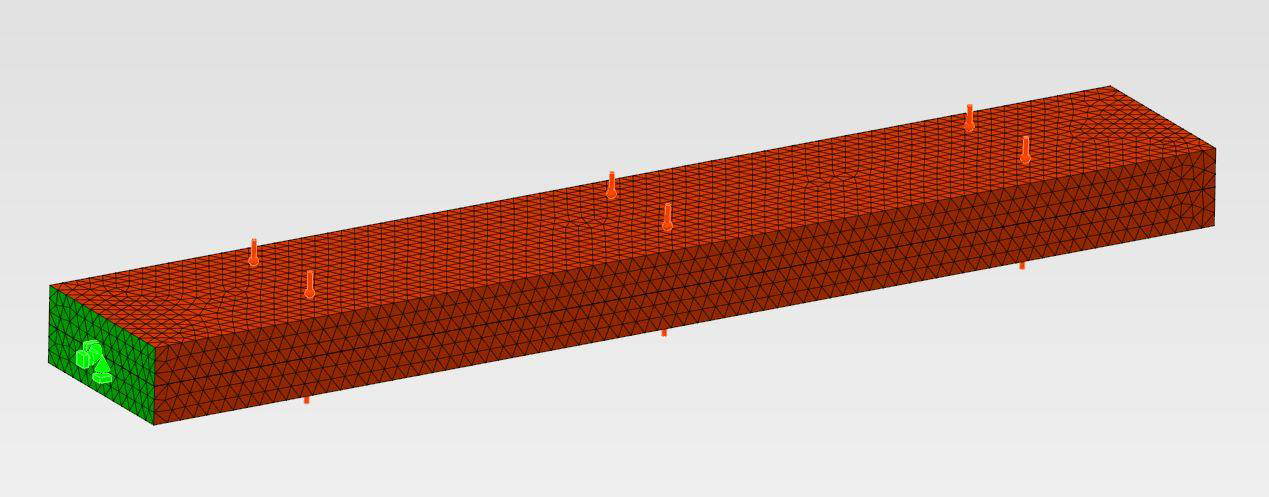
\includegraphics[width=140mm]{fig/12-02.png}
	\caption{バイメタル小片 - 境界条件}
	\label{fig:12-02}
	\end{figure}
	\vspace{-\baselineskip}
\item
  必要な定義がすべて行われたので、解析を提出できます。
  解析が終了するまで待って、結果を開きます。
\item
  垂直変位のコンタープロットを調べます(図37)。
  分析的に計算されたバイメタル小片のたわみは0.3807mmです。
  解析では、これよりも若干高い予測値が得られることがあります。
	\begin{figure}[H]
	\centering
	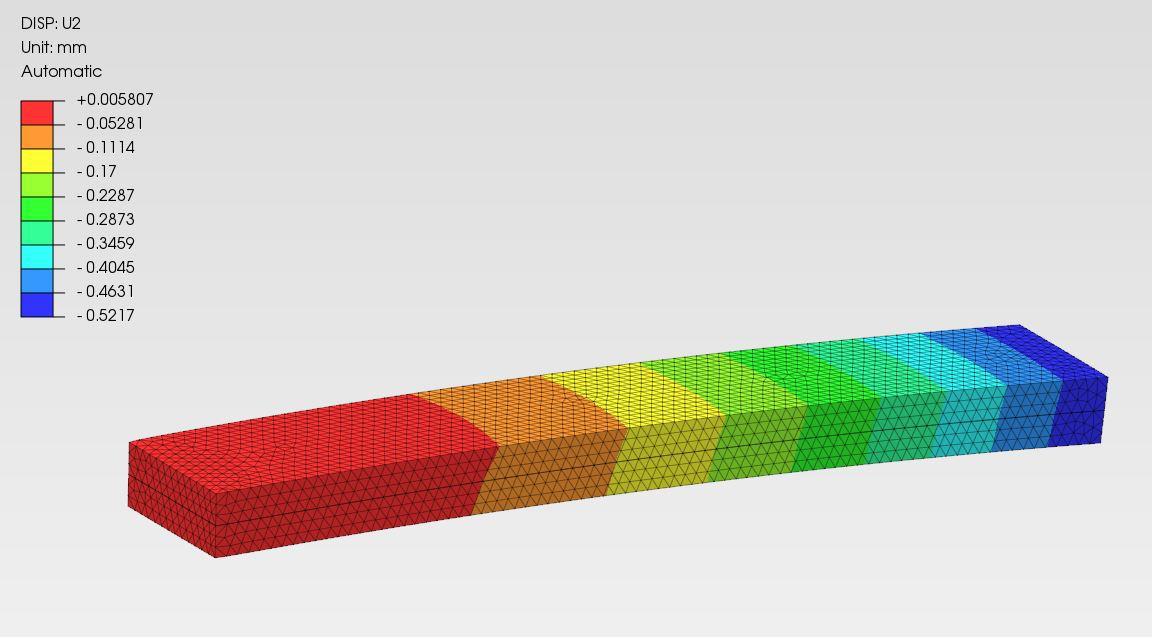
\includegraphics[width=145mm]{fig/12-03.png}
	\caption{バイメタル小片 - たわみ}
	\label{fig:12-03}
	\end{figure}
\end{enumerate}